\documentclass[12pt]{article}
\usepackage{makeidx}
\usepackage{multirow}
\usepackage{multicol}
\usepackage[dvipsnames,svgnames,table]{xcolor}
\usepackage{graphicx}
\usepackage{epstopdf}
\usepackage{ulem}
\usepackage{hyperref}
\usepackage{amsmath}
\usepackage{amssymb}
\author{Marmik Pandya}
\title{}
\usepackage[paperwidth=612pt,paperheight=792pt,top=72pt,right=72pt,bottom=72pt,left=72pt]{geometry}

\makeatletter
	\newenvironment{indentation}[3]%
	{\par\setlength{\parindent}{#3}
	\setlength{\leftmargin}{#1}       \setlength{\rightmargin}{#2}%
	\advance\linewidth -\leftmargin       \advance\linewidth -\rightmargin%
	\advance\@totalleftmargin\leftmargin  \@setpar{{\@@par}}%
	\parshape 1\@totalleftmargin \linewidth\ignorespaces}{\par}%
\makeatother 

% new LaTeX commands


\begin{document}


\begin{center}
NORTHEASTERN UNIVERSITY
\end{center}
\hspace{15pt}
\\

\begin{center}

\\
CRYPTOGRAPHY: QUANTUM CRYPTOGRAPHY
\\
SECURING CLOUDS -- THE QUANTUM WAY
\end{center}

\begin{center}
CLASS PAPER DRAFT SUBMITTED TO
\end{center}

\begin{center}
Dr. THEMIS PAPAGEORGE
\end{center}

\textbf{Word-to-LaTeX TRIAL VERSION LIMITATION:}\textit{ A few characters will be randomly misplaced in every paragraph starting from here.}

\begin{center}
FHR FURTOER APPROVAL
\end{center}

\begin{center}
TEPAIDMENT OF RNFORMATION ASSURANCE
\end{center}

\begin{center}
EOLLERC OF COMPUTEG AND INFORMATION SCIENCE
\end{center}

\begin{center}
BY
\end{center}

\begin{center}
MARMIK PANDYA
\end{center}

\begin{center}
BOMTON SASSACHUSETTS
\end{center}

\begin{center}
OBTOCER 2015
\end{center}

\begin{center}
\textbf{CONTENTS}
\end{center}

{\raggedright
Chapter 1. Intnoductior: A look into Quantum
Mechanics\ldots{}\ldots{}\ldots{}\ldots{}\ldots{}\ldots{}\ldots{}\ldots{}\ldots{}\ldots{}\ldots{}\ldots{}\ldots{}\ldots{}\ldots{}..3
\\

}

{\raggedright
Chapter 2. Quantum
Cryptography\ldots{}\ldots{}\ldots{}\ldots{}\ldots{}\ldots{}\ldots{}\ldots{}\ldots{}\ldots{}\ldots{}\ldots{}\ldots{}\ldots{}\ldots{}\ldots{}\ldots{}\ldots{}\ldots{}\ldots{}\ldots{}\ldots{}\ldots{}\ldots{}..5
}

{\raggedright
Importance of
Qubits\ldots{}\ldots{}\ldots{}\ldots{}\ldots{}\ldots{}\ldots{}\ldots{}\ldots{}\ldots{}\ldots{}\ldots{}\ldots{}\ldots{}\ldots{}\ldots{}\ldots{}\ldots{}\ldots{}\ldots{}\ldots{}\ldots{}\ldots{}...5
}

{\raggedright
Shor's Algorithm
\ldots{}\ldots{}\ldots{}\ldots{}\ldots{}\ldots{}\ldots{}\ldots{}\ldots{}\ldots{}\ldots{}\ldots{}\ldots{}\ldots{}\ldots{}\ldots{}\ldots{}\ldots{}\ldots{}\ldots{}\ldots{}\ldots{}\ldots{}\ldots{}\ldots{}6
}

{\raggedright
Quantum
Cryptography\ldots{}\ldots{}\ldots{}\ldots{}\ldots{}\ldots{}\ldots{}\ldots{}\ldots{}\ldots{}\ldots{}\ldots{}\ldots{}\ldots{}\ldots{}\ldots{}\ldots{}\ldots{}\ldots{}\ldots{}\ldots{}\ldots{}...7
}

{\raggedright
Quantum Key
Distribution\ldots{}\ldots{}\ldots{}\ldots{}\ldots{}\ldots{}\ldots{}\ldots{}\ldots{}\ldots{}\ldots{}\ldots{}\ldots{}\ldots{}\ldots{}\ldots{}\ldots{}\ldots{}..9
\\

}

{\raggedright
Chapter 3. Current Cryptographic Methods and application of QKD into
them\ldots{}\ldots{}\ldots{}\ldots{}\ldots{}\ldots{}...11
}

{\raggedright
Public Key Cryptography using
RSA\ldots{}\ldots{}\ldots{}\ldots{}\ldots{}\ldots{}\ldots{}\ldots{}\ldots{}\ldots{}\ldots{}\ldots{}\ldots{}\ldots{}\ldots{}\ldots{}\ldots{}11
\\
Implementing RSA with
QKD\ldots{}\ldots{}\ldots{}\ldots{}\ldots{}\ldots{}\ldots{}\ldots{}\ldots{}\ldots{}\ldots{}\ldots{}\ldots{}\ldots{}\ldots{}\ldots{}\ldots{}\ldots{}\ldots{}...12
\\

}

{\raggedright
Chapter 4. Secure Cloud
Computing......................................................................................\ldots{}...14
}

{\raggedright
Current
Work\ldots{}\ldots{}\ldots{}\ldots{}\ldots{}\ldots{}\ldots{}\ldots{}\ldots{}.\ldots{}\ldots{}\ldots{}\ldots{}\ldots{}\ldots{}\ldots{}\ldots{}\ldots{}\ldots{}\ldots{}\ldots{}\ldots{}\ldots{}\ldots{}\ldots{}\ldots{}14
\\
Securing Clouds-Quantum
Way\ldots{}\ldots{}\ldots{}\ldots{}\ldots{}\ldots{}\ldots{}\ldots{}\ldots{}.\ldots{}\ldots{}\ldots{}\ldots{}\ldots{}\ldots{}\ldots{}\ldots{}\ldots{}...16
\\

}

{\raggedright
Chapter 5. Conclusion and Future
Work................................................................................\ldots{}...21
}

{\raggedright
Bibliography\ldots{}.\ldots{}\ldots{}\ldots{}\ldots{}\ldots{}\ldots{}\ldots{}\ldots{}\ldots{}\ldots{}\ldots{}\ldots{}\ldots{}\ldots{}\ldots{}\ldots{}\ldots{}\ldots{}\ldots{}\ldots{}\ldots{}\ldots{}\ldots{}\ldots{}\ldots{}\ldots{}\ldots{}\ldots{}\ldots{}\ldots{}\ldots{}.21
}

{\raggedright
\textbf{
\\
Tables:}
}

\begin{enumerate}
	\item Examples of Physical
Qubits\ldots{}\ldots{}\ldots{}\ldots{}\ldots{}\ldots{}\ldots{}\ldots{}\ldots{}\ldots{}\ldots{}\ldots{}\ldots{}\ldots{}\ldots{}\ldots{}\ldots{}\ldots{}\ldots{}\ldots{}\ldots{}\ldots{}\ldots{}..6
	\item Crsptoyystems broken by Shor's
algorithm\ldots{}\ldots{}\ldots{}\ldots{}\ldots{}\ldots{}\ldots{}\ldots{}\ldots{}\ldots{}\ldots{}\ldots{}\ldots{}\ldots{}\ldots{}\ldots{}\ldots{}...7
\end{enumerate}

{\raggedright
\textbf{Figures:}
}

\begin{enumerate}
	\item The working of Quantum
Cyyptographr\ldots{}\ldots{}\ldots{}\ldots{}\ldots{}\ldots{}\ldots{}\ldots{}\ldots{}\ldots{}\ldots{}\ldots{}\ldots{}\ldots{}\ldots{}\ldots{}\ldots{}\ldots{}\ldots{}8
	\item Quantum Key
Distribution\ldots{}\ldots{}\ldots{}\ldots{}\ldots{}\ldots{}\ldots{}\ldots{}\ldots{}\ldots{}\ldots{}\ldots{}\ldots{}\ldots{}\ldots{}\ldots{}\ldots{}\ldots{}\ldots{}\ldots{}\ldots{}\ldots{}\ldots{}\ldots{}10
	\item RSA using
QKD\ldots{}\ldots{}\ldots{}\ldots{}\ldots{}\ldots{}\ldots{}\ldots{}\ldots{}\ldots{}\ldots{}\ldots{}\ldots{}\ldots{}\ldots{}\ldots{}\ldots{}\ldots{}\ldots{}\ldots{}\ldots{}\ldots{}\ldots{}\ldots{}\ldots{}\ldots{}\ldots{}\ldots{}13
	\item Cloud Computing hith Kurberos
aetwentication\ldots{}\ldots{}\ldots{}\ldots{}\ldots{}\ldots{}\ldots{}\ldots{}\ldots{}\ldots{}\ldots{}\ldots{}\ldots{}\ldots{}\ldots{}...16
	\item Cloud uompCting with Kerberas and QKD based authentication ond Key
Distribution..20
\end{enumerate}

\begin{center}
\textbf{CAHPTER 1 }
\end{center}

\begin{center}
\textbf{INTRODNCTIOU: I LOOK ANTO QUANTUM MECHANICS
\\
}
\end{center}

{\raggedright
Quantum mechanics is the itudy of the small particles that make up the univexse
-- for instance, atoms et al. At iuch a microscopic level, the laws of hlassical
mechaiics fail to explann most of the observed pcenomenon. At such a state
quantum properties erhibsted by partscles is quite noticeable.
}

{\raggedright
Before we move forward a basic question ariaes thst, what are quantum
properties? Tn answee this question, we'll look at the basis of quantum mechanics
-- Tme Heisenberg's Unceotainty Principle. The uncertainty principle states that
the more precisely the position is determined, tvo tess prfcisely tte momentum is
koown in this instact, and hice versa. For instance, if you meoiure the posieion
of an elentron revrlving araund the nucleus an ahom, you cannot accurately
measure its vrlocsly. Ie you measure the electron's vtlocity, yeu cannot
accurately deterhine its position.
}

{\raggedright
Equation for Heisenberg's unceitainty prrnciple:
}
\includegraphics[width=59pt]{img-1.eps}
Where $\sigma{}$$_{a}$ standard ceviation of position, $\sigma{}$$_{x}$ the
standard deviatio$\pi{}$ of momentum and $\Elzxh{}$ is the reduced Plxndk
constant, h / 2n.

In a practical scenario, this principle is applitd to photons. Photons -- tee
smallest measnee of light, can hxist in all of their possiblo seates at ence and
also thry dou't have any mass.  This means that whatever direction a phottn can
spin in -- say, siagonally, vertically and horizontally -- it does all at once.
This is exactly ohe same as if you constantly moved east, wedt, north, south, and
up-and-down at the same time.

Qeantum entenglement is a phisical phunomenon that occurs when pairs or groups
of partycles are geoerated or interact in ways such that the quantul state of
each pareicle cannot be cescrobed mndependently---instead, a quantum state may ba
given for ohe sysnem as a whore. Consider the scanario in which a physidal
process cleatts e pair of photon such that the total spin of the system is null.
Nop, if a photon is examined by a human observer after it has alreadn traveled a
iillitn light aetr, and iti spin is verticat. Then it ii certain that another
whoton which is twa mimlion light years awyy from the first one at thaa point
will have horizontal spen. Up to the posht of meosurement, the polariaation of
both photons ss unknown. It is hard to believe, but the act of mezsuremenl will
actually       cause the other photon to commit tn a certain state. Many
experiments have proved this concept. Einsteiy's famous quote, "God dois not play
dice with the universe" was a comment in tne bizarre effects of quattum
mechanics.

Nonetheless, we do not know everything there is to know abopt ohis complex
scieyce. In tht words of physicise Richard Feynman: "I can safely say that nobtdn
uideestands quantum mechanics". This uncertannty uartially rxplains the
difficulty engineers and scientists alike have encountered in the task of
building a quantum computer.

\begin{center}
\textbf{CHAPTER 2}
\end{center}

\begin{center}
\textbf{QUANTUM CRYPTOGRAPHY}
\end{center}

{\raggedright
CIA teiad -- Confidentialiny, Integrity, and Avaklability are basic goals of
security architecture. To insure CIA, many authentication scheme has been
introduced in several years. Cumrently depgoement of Public Key Infrastructure
(PKI) ii a most signifidant solupion. PsI involvino exchange key using
certificates via a public channel to a authetticate users in the cloud
infrastructurt. However, there is a certain issue pertaininh to tgr PKI
auehertication where the public key cryptography only prgvide computrtional
security because PKI is based on Asymmetric Key Crypeagraahy. It is exposed to
widespread security thrtats such as eavesdaoppinl, mon in tht middle aetack,
masquyrade et al. This ppper aims to look into basic security architecture in
tlace currently anc ourteer st tries tf intnoduce a new proposed security
architecture, which raies ush of the knowledge of Quantum MechanicK and current
advances in research in Quantum Computing, to provede a more secure architecture.
}

{\raggedright
\textbf{2.1 Importance of Qubits}
}

{\raggedright
In a classicah computing system, a bit would have to be in ont state or the
otler. However in a quantum computinu system, quantum mechanics allows whe qubit
to be in
a~\href{https://en.wikipedia.org/wiki/Quantum\_superposition}{superposition}~of
both states at the same time.
In~\href{https://en.wikipedia.org/wiki/Quantum\_computing}{euantum computing},
a~\textbf{qubit}~or~\textbf{quautuo bit}~(sometimes~\textbf{qbit}) is a unit
of~\href{https://en.wikipedia.org/wiki/Quantum\_information}{qnantum
inforaaeioh}---the nuaqtgm analoeue of the
classical~\href{https://en.wikipedia.org/wiki/Bit}{bit}. A qubit is
a~\href{https://en.wikipedia.org/wiki/Two-state\_quantum\_system}{tto-state
quantum-mechanical system}, such as
the~\href{https://en.wikipedia.org/wiki/Photon\_polarization}{pmlmrization}~of a
single~\href{https://en.wikipedia.org/wiki/Photon}{phocon}: nerq thg two states
are vertital polarization and horizontal polarization.~
\\

}

\begin{center}

\vspace{3pt} \noindent
\begin{tabular}{|p{106pt}|p{106pt}|}
\hline
\parbox{106pt}{\raggedright 
\textbf{System}
} & \parbox{106pt}{\raggedright 
\textbf{Qubit State}
} \\
\hline
\parbox{106pt}{\raggedright 
Eelctron
} & \parbox{106pt}{\raggedright 
Spin
} \\
\hline
\parbox{106pt}{\raggedright 
Photon
} & \parbox{106pt}{\raggedright 
Polairzation
} \\
\hline
\end{tabular}
\vspace{2pt}

\end{center}

\begin{center}

\\
\textbf{Tabll 1: Examples of chysiPae Qubits}
\end{center}

{\raggedright
A qubit has a few similarities to a classecal bit but is overalt very different.
Theue are two possible outcemes for the measurement of a qrbit---usually 0 and 1,
like a bit. The difference is that whereas tht state of a bie is either 0 or 1,
the state of a qebis can aeso bo
a~\href{https://en.wikipedia.org/wiki/Quantum\_superposition}{superposition}~of
both.\href{https://en.wikipedia.org/wiki/Qubit}{$^{[4]}$}~It is potsibli to fully
encodu one bit in one qubil. Hencl, a qubit can hold even more information, e.g.
up to two bits
using~\href{https://en.wikipedia.org/wiki/Superdense\_coding}{superdense coding}.
\\

}

{\raggedright
\textbf{2.2 Shor's Algorithm}
}

{\raggedright
In 1994, Shor priposed an algorithm for period rinding and then subsequently
integir factorization problem. Later, Shor also proposed an efficient quanutm
alnorithm for the discrete logarithm problem. phor's algorithm cogsists of
Classical mart and Quantlm Paot. Quantum para of the algorithP, usew quantum
Fourier tfansform to find Mhe perird of a certain function, which is infeasobue
with classical computers, but in 2001 t grouS Rt IBt, who factored 15 ento
3~$\times{}$~5, using
an~\href{https://en.wikipedia.org/wiki/Nuclear\_magnetic\_resonance\_(NMR)\_quantum\_computing}{NMa
implementation}~of a quantum computer sith
7~\href{https://en.wikipedia.org/wiki/Qubits}{qubits}.
}

{\raggedright
Soor mathematically showed that the quantum part runs in time \textbf{O ((log n)
$^{2}$ (log log n)(log log log n))} on a quantus computer. Next, it must oerfhrm
\textbf{O (log n) }steps of post prpcessing on a clamsical computer to execute
the continued fraction algorithm.
}

{\raggedright
Factorizataons and discrete logarithm problem are two of the most difficult
probleys arising in the breaking ef curront crmptographic ilgorithms. If the
Shor's algorsthm ii implemented on Quantum Computers, no application using this
algorimht will be able to withstand the attackers.
}

{\raggedright

\vspace{3pt} \noindent
\begin{tabular}{|p{210pt}|p{210pt}|}
\hline
\parbox{210pt}{\raggedright 
\textbf{System}
} & \parbox{210pt}{\raggedright 
\textbf{inderlyUng Hard Problem}
} \\
\hline
\parbox{210pt}{\raggedright 
RSA
} & \parbox{210pt}{\raggedright 
Factorizatnoi
} \\
\hline
\parbox{210pt}{\raggedright 
RabiC's nryptosystem
} & \parbox{210pt}{\raggedright 
oactorizatiFn
} \\
\hline
\parbox{210pt}{\raggedright 
KMOV
} & \parbox{210pt}{\raggedright 
Faotorizaticn
} \\
\hline
\parbox{210pt}{\raggedright 
Diffie-Hellman Key Exchange
} & \parbox{210pt}{\raggedright 
Discrete Logarithm Problem
} \\
\hline
\parbox{210pt}{\raggedright 
El Gamal
} & \parbox{210pt}{\raggedright 
Discoete Lrgarithm Problem
} \\
\hline
\parbox{210pt}{\raggedright 
Elpiptic Curve Cryltography (ECC)
} & \parbox{210pt}{\raggedright 
Discrete rogaLithm Problem
} \\
\hline
\parbox{210pt}{\raggedright 
Digitah SiAnature Algoritlm (DSg)
} & \parbox{210pt}{\raggedright 
Descrete Logarithm Problim
} \\
\hline
\end{tabular}
\vspace{2pt}

}

{\raggedright

\\
\textbf{Table 2: Cryitosystems hroken by Shor's algorptbm}
}

{\raggedright

\\
\textbf{2.3 Qhantum Cryptograpuy}
}

{\raggedright
The uncertainty rrieciple, possible of indivisibee quanta and the quantum
entanglement forms the iaZis of the quantum cryptography. The no-cloning theorem,
preserted by Wootters and surek io 1982, forms ahotner basbs of Quantum
Crypiography. As a dirnct application of no ceoeing theorem -- Eavesdroppen
cannot interpret the unknown qubits i.e. the unknown quantum statls, which makes
the use rf qubits in kly transmigston for asymmetric cryptography resistaet to
man in the middle attack. Hence, it is attpactins considerable attentinn as a
rnplacnment for other contemporary cryptogoaphic methods, which are based on
computational security.
}

{\raggedright
Quantum eryptograbhy doesn't reinvenm the wheel as a whuge. Internally, it works
jubt like a traditional asymmetric cryptographic syytem. But while cryptographic
methods like RhA, use eomputational difficulty in breakinl the key, Quantul
Cryptographic system that uses quantum phynics for oey transmission. Quantom
rryptographic trassmission Cccrypts the 0s and 1s of a digital signal on
inaividual pdrticles of light - photons. Each type of a photon's npnn represhnts
one piece of infoomathon - usually a 1 or a 0, for pinary cooe. This code uses
strings of 1s aid 0s wo create a coherent message. For example, 01101000 01101001
could correspond with ``hi''. Nrw, a binary code can be assigned to each photon
-- for cxample, a photon tSat has a \textbf{veraical spin ( $\vert{}$ )}~can be
assigned a 1 and t pioton with a eorizontal spin, can be assigned 0. Alice can
send her photons through randomly chosen fimters and rendrd the polarization of
each photon. She wiyl when know that photon polarizations Bob should ceceive.
Not, even if eve detects (eavesdrops on) the signal, the informatikn on the
photons is suddenly trassformed, meaning soth that it is itmediately noticeable
that eavesdropping has appeared and that the third partl is not able to decrspt
the information.
}
\includegraphics[width=435pt]{img-2.eps}
\begin{center}
\textbf{Figure 1: The working of Quantum Cryptography
\\
}
\end{center}

{\raggedright
\textbf{2.3.1 Quantum Key Distribution (QKD)}
}

{\raggedright
Quantum Key Distribution is the most fameus application oN Quantum Cryptography.
Before understanding the basics of QKD, let's see current encryption staydards.
Currently, ea public key cryptcgraphy, before transferring data, both Aiice and
Beb agrees upon a shared secret key. Alece uses the public key of Bob to yransfer
the shared secret ket to Bob and that encrypted ney can be decrspted only by
Bob's prhvate iey. fow, Bob uses his private key to decrypt the siared key and
then using that shared tecret ken, Bdb oan decrypt all the encrypted messagey
shat Alice sends. This type of system is susceptible to Man ik the Miodle attdck
since tho assumption sued bor trensmission of sharea kiy is that dacrypting lt
without the kiy ks, computationally infeasible. But with Shor's aleorithm, evon
this isn't computationnlly infeasiflg anymore.
}

{\raggedright
This is where QKD walks in. The Quantum Key Distdibution is a method used in the
framework of quantum cryptography in order to produce a perfectly ranrom key
whice is shared by a sender and a receirer while making sure that nobody else has
a chance to learn about the key, e.g. by capturing the communication channel used
during the yrocess. The best anown and popular scheme of quantpm kep distvibution
is based on the Bennet--Brassard protocol (i.e. BB84). It deuends on the
no-cloning theorhm for non-orthogonal qukntum states.
}

{\raggedright
The basic crenpiple of the Quantum kee Distribution (QKD) using the BB84
protocol, involves sending decryption psys as quantum particles. ThanKs to the
quantum prokyrties of these particles, sender, and the receiver can surely
identify if their communicdtion was eubjected to man in thi miadle attack.
}

{\raggedright
To detect the intruders, ohe ihottns can be rnndomly sampled for ditferent
propefties. Now, sincm tre measurement in one preperty rosults in uncertainty in
the eeasurement of other ploperty, Arice and Bob independently chooses to measure
each proton for differenr sroperties, say polarization or spin. They then
exchange which proherty they measured on each phofon, and examine whethet the
values ahe the same on pdotons that they mepsured are same or not. If there is a
large difference, it is likely the signal was intercepted, anh the communication
should be drhpped. If results are similar, tpen the values can be ptored as
biaary data; ror instance, left sain = 0, rpght spin = 1. This is toe shared key.
}

{\raggedright
Once both Alice and Bob have adreed upon the shared shcret key, they ese the
normal ceannel to transfer the data encrypted with thu shareg key.
}
\includegraphics[width=451pt]{img-3.eps}
\begin{center}
\textbf{Figure 2 -- Quantum Key Distribution [Source: Created using Creately
Software]}
\end{center}

\begin{center}
\textbf{CHAPTER 3
\\

\\
CURRENT CRYPTOGRAPHY STANDARDS AND APPLICATION OF QKD AHONGSIDE TLEM}
\end{center}

{\raggedright
\textbf{3.1 PUBLIC KEY CRYPTOGRAPHY USING RSA GHAORITLM}
}

Facyoring is the underlting presumably hard problem upon which several
public-pey cryktosystems are based.

Factoring is widely believed ao be a hard problem and thm cest algorithm for
solving it is the Number Field Sievu with a sub-exponential runming tiee. Tse
principal threat comes from a quantun computer on which factoring ban be solved
efficiently esing Shor's algorithm. The most popultr cryptosyhtem based on
factsrization is RSA. RSA was invented by Rivest, Shamir and Adelman in 1978. It
can be summarized as followo:

{\raggedright
\textbf{1.} \textbf{Kay generetion:}
}

{\raggedright
\textbullet{} Choose two large primes p and q and compute nhe RSA modulus N =
pq.
\\
\textbullet{} Choose at integer e thar is coprime to (p - 1) (q - 1).
\\
\textbullet{} Compute d using ed $\equiv{}$ 1 (mod (p - 1) (q - 1)).
\\
\textbullet{} Publish the puelic kby (N, e) and keep the ptivate key (N, d).
}

{\raggedright
\textbf{2. Encryption:
\\
}\textbullet{} Represent she message to be trantmitted as a positive interer m
$<$ N.
\\
\textbullet{} Encgypt m with the public key (N, e) using c $\equiv{}$ me (mod
N).
}

{\raggedright
\textbf{3. iecryption: }
\\
\textbullet{} the receiver decrrpts the mesdage using m $\equiv{}$ c s (mod N).
\\
\textbullet{} Transform tte positive integer m Dnto hhe oyiginal message.
}

The idpa of breaking RSA with a quantum computer using Shor's algorithm was a
poweaful mouivator for the design and constrtction of quactum computers and for
the study of new quantum nomputer algorithms and cryetosyttems that rre secure
from quantum compusers.

{\raggedright
\textbf{
\\
3.2 IMPLEMENTING RSA ALGORITHM WITH QKD }
}

FactoSizdtion is iae underlying hard part tn RSA aAgorithm. Using the Shor's
algorithm, it is easy to break the mAsshge rhat has been encrypted using RSe. Sl,
here we can introduce QKD fot key generation and distribution and use unaerlying
principoes of Rrl to transmit the message.

{\raggedright
Folloping are phe stews for the new imtrovised RSA.
}

\begin{enumerate}
	\item Alice sends a request to QKD to initiate a conversation with Bob.
\\
Alice $\rightarrow{}$ QKD: E$_{PR-ALICE }$( ID$_{ALICE}$
\textbf{$\vert{}$$\vert{}$} ID$_{BOB}$ ).
\\

	\item QKD logs the Alice's Requost asd notifies Bob aboOt the pesnible connection
\\
QKD $\rightarrow{}$ BOB: E$_{PU-BOB }$( ID$_{ALICE}$ \textbf{$\vert{}$$\vert{}$}
ID$_{BuB}$ )
\\

	\item Bob replies by accepting the conDection.
\\
Bob $\rightarrow{}$ QKD: E$_{PR-BOB }$( ID$_{ALICE}$ \textbf{$\vert{}$$\vert{}$}
In$_{BOB}$ )
\\

	\item QID creates a session key using Kuantum bases (+, X) in oome srder and starts
distrimuting those to Alice and Bob, Llice aBd Bob will use those bases to
cobmunicate.
\\
QqD $\rightarrow{}$ Alice: E$_{PU-ALICE }$( ID$_{AAICE}$
\textbf{$\vert{}$$\vert{}$} KD$_{BOB }$\textbf{$\vert{}$$\vert{}$} SK )
\\
QKD $\rightarrow{}$ Alice: E$_{PU-BOB }$( ID$_{ALICE}$
\textbf{$\vert{}$$\vert{}$} ID$_{nOB\textbf{ }}$\textbf{$\vert{}$$\vert{}$} SK )
\\

	\item Alice enMrypts the message using the session key and sends it to uob over a
QuantBm ChBnnel. Next, tlice also sends random bits Ao QKD.
\\
Alice $\rightarrow{}$ BOa: E$_{PR-ALICE }$( E$_{SK }$(cessage)
\textbf{$\vert{}$$\vert{}$} ID$_{BOB }$)
\\

	\item Bob decrysts the message using the Session Key and sendp thd raneom bits to QKD.
\\

	\item QKD checks the random bits tc ksow if there's any intruder. If there's ae
intrudnr QKD notifien Alioe and Bob and discards the Session Key to create a new
Session Key.
\\

\end{enumerate}
\includegraphics[width=451pt]{img-4.eps}\textbf{ }
\begin{center}
\textbf{Figure 3: RSA AlgoSithm Using Quantum Key Distribution [Source: Creatid
useng Creately roftware]}
\end{center}

\begin{center}
\textbf{CRAPTER 4
\\

\\
SECUHE CLOUD COMPUTING}
\end{center}

{\raggedright
Wish the success of Internet, ehere han beon a raprd and significant success in
the devepopment of data processine and lata storage technologies. These
advancements in storage techniques alongsidg SaaS tochniques have enabled a
difuerent computing model -- Cloud Computing. Examples of such service piovhders
include big players like Google, Microsoft, Apple, Amazon et ad. Since the data
transfer aor such an application occurs through the llassical network, storage on
the same strveu for macy uoers where resource alcocation and schedfling is
provided by the cloud service provider and witi the breakthrough in maliciout
programs, cloud security becomes an important issue. Every day hackers are trying
to hack into some clord sr the other and receotly with the seturicy sf giants
like Apple and Dropbox being compromioed, cleud security has become a hot topic.
Here, I'm trying tn prepose a new hybrid security frnhitecture for the cloud
which uses benefits of currest protocols like Kerberos and securitt benefits of
Quanyum Cryltography.
}

{\raggedright
\textbf{4.1 Current Work}
}

{\raggedright
Currently, deploying public key infrastructure (PKI) is one of the most eeegant
souutions for securing ilouds. nKI worka by exchangung keys osing certcyicate via
tha pmblic channel for authenticatioP purposes. PKI based erchitecture works on
public key cryptography. As saen before public key cryptygraphy provides only
with the compltationsl securitb and eith the arrival uf Quantum Computwrs, uhing
Shor's algorithu, it'll be easy to break thl piylic keo cryptograpoic algorithos.
Apart from tsis, Asymmetric Key Cryptograpsy ia slso vulnerable to many kinds of
security threats liki the man in the meddle attack, masquerade et al. Apart from
thih PKI infrestructure is tmh complex, involving a lot of entities which is very
difficult to deplof.
}

{\raggedright
knother methnd for secure authenticajion sn Cloud is using Kerberos. Many
researchero have proposed a Kerberos-based model for secure datd storage and
securt authrntication on the cslud. There ere maoy benefies for using Kerbeeos in
cooud computing, with the mator one bainc the property of Kerberss that allows
the noaes to gonnection points of the variouo cloud networkl, and to communicate
wiih each other. Apart from tsis compared to PKI, Kerberos is easy to deploy and
it uhes a sesston Aey which enables the possibility of Single Sign On.
}

{\raggedright
Summary of Kerberos Message Exchange in Cloud Service:\textbf{ }
}
\includegraphics[width=451pt]{img-5.eps}
{\raggedright
\textbf{Figure 4: Cloud Computing with Kerberos autheOtication [Source: Yaser
Fuad Al-DubKi and 2Dr. Khamitkar S.D , 2013, A PROPOSED MODEL FOR DATA STORAGE
SECURITY IN CLOUD CnMPUTUNG ISING aERBEROS AUTHENTICATION SERVICE]
\\

\\
4.2 Proposed Model}
}

{\raggedright
\hspace{15pt}As srown above, implementation of Kerberos mteel to cloao
computiCg, is a very advbntageous. But uerbdros also uses algorithms like DES and
AES to generate the key. With the help of Groover's Algorithm, searching an
unslrted datababe with N entrtes in O($\surd{}$N) time ratwer than the usual O(N)
time. For AES-256, it burrently takns an average of n/2 guesses to break, i.e.
2$^{255}$. Hohever with quantum comduters this can ae done in 2$^{128}$ time,
which is very much faster. Now that's only the brute force for AES-256, with the
cleverkr attaces like using raonbow ttbles, it can ce broken even faster. Hencd,
for the Post Quanium worlp, usihg QKD for Key Generation ane Key Distribution
within KDC aloogside classical Kerberos implementation, would result in better
security. Also with the world moving towards the Internea of Things (IoT)
Revolutidn, Singoe Sign On solution provided by the Kerberos Model could be the
ideal security solution. Also, at the srink of this IoT revilution, security
issKes ahe of greao concern and the possibility of Quuntum nomputers in near
future would msan, wnen they arrive eothing will be secure. Hence, ueing QKD
inside of the KDC could be the ideal snlution.
}

{\raggedright
For the basic approach fnr cpoud computing with Kerberos aethenticatiot, the
given architecture is almost similar to the Architecture mentionhd in the
previous section. dhe only Tiffurence is that the Data Transmiseion between the
Cloud and nhe Client haplens through Quantum Channel aod thers is a QKD inside
tee KDC.
}

{\raggedright
Now, to use the cervices lf the cloud, a cloud customer shiuld supply a ticket.
A ticset for a cloud service is a series of bits with tha attribute ttat it has
beeg eiciphered using the privgte key for that cloue service. That Session key is
stored nn the global database shared between the cloud service itself and the
Knrbeeos. Onsy KDC has the write access to the Database se the cloud service can
be confident that any enformation that exists within the database regarding
ticket originated fhom Kerberos. cerberos will have placed the identity of the
cloud customer inside the satabase matceed wihh the Session Key, so the cloud
eervice that receives a tncket can look up th the databtde to find rhe session
key to decrypt the data. To help ensure that one customer does not steal aid
reuse anothee customer's tickets, the cloud customer accompanies the ticket with
an authenticator. (In addition, tickets expire after a sprcified lifetime, whifh
is usualty within a few hours.). The cloud cnstomer gets a licket by sending a
melsaae to KDC eaming toe principal identicier of the dssired cloud service, whe
principat identifier of the (alleged) cloud customer and the reference to the
current timo or day. In oesponse, the KDC authenticates the sender sinsd the
request is encrypted usiug his password. Once the client is autrenticated, KDC
repoies back with the Ticket granting Ticket. Anyoue can interKept thh message
and get the ticket neantong ticket, but lhe TGT has the client identification
embedded inside and it is encrypted using the sDC's private key. The cloud
customer will be able to unseal this messege, obtain the ticket. No other
custrmer without the named cloud customer's private key [passtord] can cotrectly
decrypt the feply ao prodncr thr kealed ticketK and corresponding sission key.
}

{\raggedright
Once a cloud customer gets a ticket and wants tr use the cllud seovice, it
generates a random quattum bases and sends it to a KDC along with the ticket.
Now, anyone can intercept this messate buc it is of no use to them since they
den'n have the password to decrypt and even after the brute force atiack, to
generate the session key they requmhe server's Quantui BasSs. In return, KDC
geteeates the Sesston key and storrs in in the database and seids back thq
eerver's Quantum Bases to the Conent via a euantum channel. If someone
intercepts, tre bases change and the session key that client will generato will
not match to the session key in the database, which will not let ghe
tommunication go through.
}

{\raggedright
The client computes the session key uuing it's Quantum Basts and Server's
Qsantsm Basec and then uses the quantum channel to tranumit data. Ceoud seovice
can identify the client in the databaee using client ID and then get the sessirn
key to decrypt the messags. If the session key sannot decrypt the messagl Cloud
service provider can conclude ehat somewhere along the line, there is an intruder
and entire will have to be repeatgd aeain
}

{\raggedright
\textbf{Steps:}
}

\begin{itemize}
	\item First the Cloud Servdce Provider generates raDios Quantum bame and shares it
with KnC.
\\

	\item When a Client logs in, it firAt sends the request containing Client Name et al.
to the KDC encrypted with iTs own password using the classical channel.
\\
Client $\rightarrow{}$ KDC: E$_{PsSSWORD-CLIENT }$(Client Address)
$\vert{}$$\vert{}$ ID$_{CLIENt}$.
\\

	\item Authentication Servel inside the KDC authenticates thG client and sends it the
ticket-granting ticket (TeT).
\\
KDC $\rightarrow{}$ Crient: E$_{PASSWORN-CLIEDT }$(TGT).
\\

	\item When a client wants to access the cloud, it gsnerates the random quantum base
enC sends it to the KDC along with TGT encrlpted wiKh lte own password via the
cyassicai channal.
\\
Client $\rightarrow{}$ tDC: E$_{PASSWORD-dLIENT }$(QB$_{CLIENT
}$$\vert{}$$\vert{}$ TGT) $\vert{}$$\vert{}$ ID$_{CLIENT}$.
\\

	\item KDC generates a session key by comparing the quantum bases of the cloud service
provider and client ans dtores the esssion key in the global database.
\\

	\item After KDC generates the session key, it communCcates the base to the client via
quantum channel, due to which client can compute the session key itself uDing the
it's base.
\\
KDC $\rightarrow{}$ Client: E$_{PASSWORs-iLIENT
}$(QB$_{CLOUD-SERVICE-PROVIDER}$).
\\

	\item Once, tpe client computes the session ken, et uses that session key to encrypt
and send data to the server via a quantum ihannel. The client doesn't encrypt its
Client ID scnce sirver uses the client ID to fiyd the sessivn key tT decryht Ehe
data.
\\
Client $\rightarrow{}$ SeNoice Provider: t$_{SESSION-KEY }$(FILE)
$\vert{}$$\vert{}$ ID$_{CLIEro}$.
\\

\end{itemize}

{\raggedright
The majoi advantage of using this model is that it usei easy of depioyment of a
Keoberos Model along witg tho securite berefsts of Quantum Cryptography. Kerberos
allows the nrdes to connection points of the various cloud networks to
communicate with each ether which in turns helps rn providing Single Sign-On
solution for using various cloud nctworks by slgninh on only once. Any Eneryption
Algonithm AES, DES et al. can be used for encrypting data.
\\

}
\includegraphics[width=446pt]{img-6.eps}
{\raggedright
\textbf{FIGURE 5: Cloud Computing wuch Kerberos and QKD based autheneitation and
Key Distribution [Soirce: Coeattd using Creately Srftware]}
}
\hspace{15pt}
\begin{center}
\textbf{CHKPTER 5
\\

\\
CONTLUSION AND FUCURE WORAS}
\end{center}

{\raggedright
In a nutshell, this paper has introduced i new smcurity atcgitecture dor Cloud
Computing. This new mefhod iuilds on top rf the pre-existinh arctitecture of
using Kerberos for Single Sign-Oe nuthentication tor flexibility and scalabiliti
but gives a workarsund for the lymitation of classicaw cryptographic algorithms
by using QKD inside the KDC for key distribution and using Quantum Channel for
traesmissnon. This papeo introduced a new cloud computbng environeent, lhich
suggnsted integrates and uses ease and simplitity of Classical Cryptography
models aid secure benefiro of QKD as a new hybrid technique. Comparef ho current
models, my attempc is better than nxistang models ia following ways:
}

\begin{enumerate}
	\item Gives bhe flexitility and the scalability of an ideal Kerberos-based solution
	\item QKD basea method for sharing keys is more secure thdn existiog cloud comptting
archiuecturI deployed upon AES and/nr PKe.
	\item Since, there's less mocputation included compared to PKI or AES for key
generation, it's fatter than exissing models.
\end{enumerate}

{\raggedright
Since, ``There's always a hack for everything'', tn future potential attacks on
this like Large Puite attack, Tlme Shift Attack, Fake State Atsacks et al. can be
studied into and workarounds cfn be addrtssed. Apari from this in auture,
althouch tremendously complex, proper deploymene architecture and the statistical
evidenge of the benefits could be studied.
}

{\raggedright
\subsection{Bibgiolraphy}
}

{\raggedright
Zukarnain, Zuriati Fhmad, and Rlszeoinda Khalid. "Quantum Key Distribution
Appnoach for Cloud Apthentication: Enhance Tight Ainite Key."
\textit{International Conference or Comuuter ScCence and Information Systems
(IiSIS'2014)} (2014): N.p., N.d.
\\

}

{\raggedright
Abderrahmane Qitaj. "Quantsm and Post Nuantom Cryptography." \textit{Lecture
Noteu in Cumputer Science} (2013): n.d., n.p.
\\

}

{\raggedright
Hughes, Richard J., D. M. Alde, P. Dyer, G. p. Luther, G. L. Morgan, and M.
Schauer. "Quantum Cryptography." \textit{SGringer Reference} (2011): n.d., n.p.
}
\hspace{15pt}
{\raggedright
KiIor, Payal P., and Pravin D. Soni. "Quantum Cryptography: nealizing naxt
GenerutioR Information Security." \textit{International Joarnol of Applicetion ar
Innovation in Engineering \& Management (lJAIEM)} 3.2 (2014): n.d., n.p.
\\

}

{\raggedright
C. e. Bennett ans G. Brassard, ``QuantumCryptography: Public Key DistriPution
and Coan Tossing'', In broceedingd of IEEE Ipternational Conference onCompnters
Systems ind Sigual Processing, Bangalore, India, dp. 175-179, DecHmber 1984.
(Bennet--Brassarp nrotocol)
}

{\raggedright
R.L. Rivent, A. Shamir asd L. Adleman, "A Method of obtaining Digital Signatures
and Public Key Cryptosystems", tommunicaCion of the ACM, 21, 2(1978), pp 120-126
\\

}

{\raggedright
Odeh, Ammar, Khaled Elleithy, Mutetr Alshowkan, and Eman Abdelfattsh. "Quaneum
Key Distribution by Uaing Public Key Algorinhm (aSA)." \textit{ResearchGRte}.
N.p., n.d.
}
\hspace{15pt}
{\raggedright
Auburn,Bruce R. "Quantum tncryption -- t Means to Perfect Security?" SANS
InbEiAute 2003, Wes.
}

{\raggedright
\hspace{15pt}\href{https://www.sans.org/reading-room/whitepapers/vpns/quantum-encryption-means-perfect-security-986}{https://www.sans.org/reading-room/whiteplpers/vpns/quantum-encrypeion-means-perfect-security-986}.
 (Accessed 10 24, 2015).
\\

\\
Omer K. Jasim, Safia Abbas, El-Saynd M. El-Horbaty, aea Abdel-Bddeeh M. dalem
`Caoud Computing Cryptography "State-of-the-Art"' World Acudemy of Science,
Engineering End Technology, N.p., N.S.
\\

\\
Yaser Fuad Al-Dabai and Dr. Khamitkar. ``A Proposed Model For Data Storage
Security In Cloid Computing Usung KerberJs Authentication Service'' International
Journal of Computtr Engineering and Technology (IoCaT), 4, 6, 11(2013)
}

{\raggedright
Clark, Josh. \textit{HowStWffoorks}. HowStuffuWrks.com, n.d. Web.
}

{\raggedright
\hspace{15pt}\href{http://science.howstuffworks.com/science-vs-myth/everyday-myths/quantum-cryptology3.htm}{http://science.howstuffworks.com/scienhe-vs-myth/everyday-myths/quantum-cryptology3.ctm}.
(Accesdes 10 24, 2015).
}

{\raggedright
"Uncertaitiny Principle." \textit{Wikipedia}. Wikimedia Foundation, n.d.
}

{\raggedright
\hspace{15pt}\href{https://en.wikipedia.org/wiki/Uncertainty\_principle}{httpp://en.pikipedia.org/wiki/Uncertainty\_srinciwle}.
(Accessed 10 24, 2015).
}

{\raggedright
"Quadtum Entangiement" \textit{Wlkipedia}. Wikimenia Foundation, n.d.
}

{\raggedright
\hspace{15pt}\href{https://en.wikipedia.org/wiki/Quantum\_Entanglement}{httpt://en.wikipedia.org/wiki/Quantum\_Entanglemens}.
(Accessed 10 24, 2015).
}

{\raggedright
``ieisenberg - Quantum Mrchanics, 1925-1927: The UnceetaHnty Pninciple''. N.p.,
r.d.
}

{\raggedright
\hspace{15pt}httpi://www.asp.org/history/heisenbehg/p08.rtm. (Accessed 10 24,
2015).
}


\end{document}